\documentclass[aspectratio=169]{beamer}
\beamertemplatenavigationsymbolsempty

\usepackage{graphicx}
\usepackage{animate}
\graphicspath{{figures/}}
\usepackage{amsmath}
\usepackage{upgreek}
\usepackage{listings}
\usepackage[english]{babel}
\usepackage[latin1]{inputenc}
\usepackage{tikz}
\usetikzlibrary{shadows.blur}
\usepackage{booktabs}
\usepackage{siunitx}

\usepackage{verbatim}
\usepackage{chemfig}
\usepackage{epstopdf}
\renewcommand*\printatom[1]{#1}
\usepackage{appendixnumberbeamer}
%\usepackage[noend]{algpseudocode}
\usepackage[version=4]{mhchem}
\usetikzlibrary{shapes.geometric}

\usepackage{subfigure}
\RequirePackage[numbers, sort&compress]{natbib}
\usepackage{multicol}
\usepackage[absolute,overlay]{textpos}
\usetikzlibrary{calc}
\newcounter{saveenumi}
\newcommand{\seti}{\setcounter{saveenumi}{\value{enumi}}}
\newcommand{\conti}{\setcounter{enumi}{\value{saveenumi}}}
\DeclareSIUnit{\calorie}{cal}
\usetikzlibrary{overlay-beamer-styles}

%%%%%%%%%%%%%%%%%%%%%%%%%%%%%%%%%%%%%%%%%%%%%
%   CUSTOM THEME DECLARATION
\newcommand{\email}[0]{astrid.boje@chalmers.se}
\usetheme{AstridChalmers}

\newcommand{\kB}{k_{\text{B}}}
\newcommand{\ka}{k_{\text{a}}}
\newcommand{\kd}{k_{\text{d}}}
\newcommand{\kf}{k_{\text{f}}}
\newcommand{\kr}{k_{\text{r}}}
\newcommand{\Ke}{K_{\text{eq}}}
\newcommand{\dGr}{dG_{\text{rxn}}}
\newcommand{\dGa}{dG_{\text{a}}}

\setbeamercolor{block body}{bg=cgreen!10}
\setbeamercolor{block title}{bg=cgreen!30}
\setbeamertemplate{blocks}[rounded]

%%%%%%%%%%%%%%%%%%%%%%%%%%%%%%%%%%%%%%%%%%%%%
%   AUTHOR AND PRESENTATION DETAILS
\title{\huge{\textbf{Title}}}
\author{Astrid Boje}
%\institute[Chalmers University]
%{
%  Chemical Physics Division\\
%  Department of Physics
%  Chalmers University of Technology
%}
\subject{Kinetics for heterogeneous catalysis}
\date{\small\today}

%%%%%%%%%%%%%%%%%%%%%%%%%%%%%%%%%%%%%%%%%%%%%
%   CUSTOM COMMANDS

\begin{document}
	
	\mytitleframe
	
	\section{First section}
	\begin{frame}{Title}
	\centering
	\begin{tikzpicture}[x=1cm, y=1cm, >=latex]
		\def\xleft{0}
		\def\xright{14}
		\def\ydown{0}
		\def\yup{7}
		\def\xmid{7}
		\def\ymid{3.5}
		\draw[draw=none, use as bounding box] (\xleft, \ydown) rectangle (\xright, \yup);
		\clip (\xleft-0.1, \ydown-0.1) rectangle (\xright+0.1, \yup+0.1);
		
		\node[anchor=north] (setup) at (\xmid, \yup)
			{Example};
	\end{tikzpicture}
\end{frame}

	
	
	\section{Acknowledgements}
	{ % these braces make the change local to the single frame

\setbeamertemplate{footline}{

\leavevmode
\centering	
\begin{tikzpicture}
\def\xleft{0}
\def\xright{15}
\def\xmid{7.5}
\def\xadj{0.1cm}
\def\yadj{0.1cm}
\node[anchor=north west] (clogo) at (\xleft, 0)
	{\pgfuseimage{chalmers-logo}};
\node[anchor=north east] (plabel) at (\xright, 0)
	{\small{Department of Physics}};

\node[anchor=west] (mailicon) at ([xshift=0.5cm]clogo.east)
	{
\includegraphics[height=0.4cm]{people/mailicon}};
\node[anchor=west, text width=0.17\textwidth, align=center] (mail) at (mailicon.east)
	{\url{astrid.boje@chalmers.se}};
	
\node[anchor=east, text width=0.17\textwidth, align=center] (web) at ([xshift=-0.5cm]plabel.west)
	{\url{https://aab64.github.io/}};
\node[anchor=east] (webicon) at (web.west)
	{
\includegraphics[height=0.4cm]{people/webicon}};

\draw[ultra thick, cnavy]
	([xshift=-\xadj,yshift=\yadj]clogo.north west) -- ([xshift=\xadj,yshift=\yadj]plabel.north east);
\draw[ultra thick, draw=none]
	([xshift=-\xadj,yshift=-\yadj]clogo.south west) -- ([xshift=\xadj,yshift=-\yadj]plabel.south east);
\end{tikzpicture}	
\vskip0pt
}

\begin{frame}[noframenumbering]{Acknowledgments}
	\centering
	\begin{tikzpicture}[x=1cm, y=1cm, >=latex]
		\def\xleft{0}
		\def\xright{14}
		\def\ydown{0}
		\def\yup{7}
		\def\xmid{7}
		\def\ymid{3.5}
		\draw[draw=none, use as bounding box] (\xleft, \ydown) rectangle (\xright, \yup);
		\clip (\xleft-0.1, \ydown-0.1) rectangle (\xright+0.1, \yup+0.1);
		
		\node[anchor=north west] (setup) at (\xleft, \yup)
			{\Large\textbf{People:}};
		
		\node[anchor=north west] (f1) at ([xshift=0.5cm, yshift=-0.75cm]\xleft, \yup)
			{
\includegraphics[height=0.2\textheight]{people/AH}};
		\node[anchor=north, text width=0.25\textwidth, align=center] (t1) at (f1.south)
			{Anders\\Hellman};
			
		\node[anchor=north east] (f4) at ([xshift=-0.5cm, yshift=-0.75cm]\xright, \yup)
			{
\includegraphics[height=0.2\textheight]{people/TB}};
		\node[anchor=north, text width=0.25\textwidth, align=center] (t4) at (f4.south)
			{Tom\'a\v{s}\\Bu\v{c}ko};

		\node[anchor=west] (f2) at ([xshift=1.7cm]f1.east)
			{
\includegraphics[height=0.2\textheight]{people/HS}};
		\node[anchor=north, text width=0.25\textwidth, align=center] (t2) at (f2.south)
			{Henrik\\Str\"om};
				
		\node[anchor=east] (f3) at ([xshift=-1.7cm]f4.west)
			{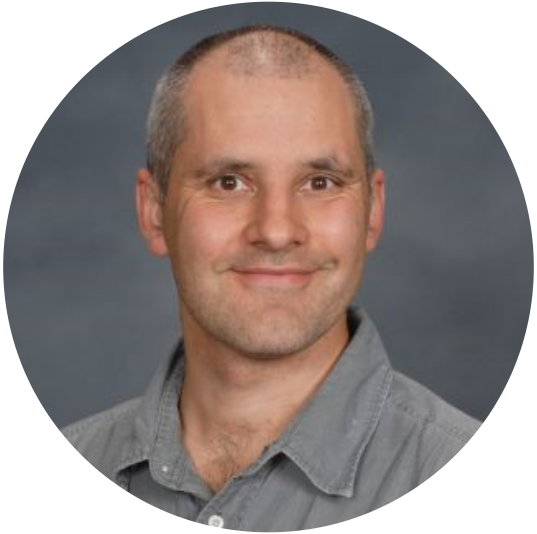
\includegraphics[height=0.2\textheight]{people/JB}};
		\node[anchor=north, text width=0.25\textwidth, align=center] (t3) at (f3.south)	
			{Jonas\\Baltrusaitis};
		
		%%%
		
		\node[anchor=north west] (setup) at ([yshift=-0.4cm]\xleft, \ymid)
			{\Large\textbf{Funding:}};
		
		\node[anchor=north west] (s1) at ([yshift=-1.15cm]\xleft, \ymid)
			{
\includegraphics[height=0.1\textheight]{sources/KAW}};
		
		\node[anchor=west] (s2) at ([xshift=0.3cm]s1.east)
			{
\includegraphics[height=0.1\textheight]{sources/SRC}};
		
		\node[anchor=west] (s3) at ([xshift=0.3cm]s2.east)
			{
\includegraphics[height=0.1\textheight]{sources/SNIC}};
		
		\node[anchor=west] (s4) at ([xshift=0.3cm]s3.east)
			{
\includegraphics[height=0.1\textheight]{sources/NSC}};
		
		\node[anchor=north] (s5) at (s4.south)
			{
\includegraphics[height=0.1\textheight]{sources/C3SE}};
		
		\node[anchor=west] (s6) at ([xshift=0.3cm]s4.east)
			{
\includegraphics[height=0.1\textheight]{sources/NSF}};
			
		\node[anchor=west] (s7) at ([xshift=0.3cm]s6.east)
			{
\includegraphics[height=0.1\textheight]{sources/xcede}};

	\end{tikzpicture}
\end{frame}
}

	
\end{document}


